\documentclass[11pt, a4paper]{article}\usepackage[]{graphicx}\usepackage[]{color}
%% maxwidth is the original width if it is less than linewidth
%% otherwise use linewidth (to make sure the graphics do not exceed the margin)
\makeatletter
\def\maxwidth{ %
  \ifdim\Gin@nat@width>\linewidth
    \linewidth
  \else
    \Gin@nat@width
  \fi
}
\makeatother

\definecolor{fgcolor}{rgb}{0.345, 0.345, 0.345}
\newcommand{\hlnum}[1]{\textcolor[rgb]{0.686,0.059,0.569}{#1}}%
\newcommand{\hlstr}[1]{\textcolor[rgb]{0.192,0.494,0.8}{#1}}%
\newcommand{\hlcom}[1]{\textcolor[rgb]{0.678,0.584,0.686}{\textit{#1}}}%
\newcommand{\hlopt}[1]{\textcolor[rgb]{0,0,0}{#1}}%
\newcommand{\hlstd}[1]{\textcolor[rgb]{0.345,0.345,0.345}{#1}}%
\newcommand{\hlkwa}[1]{\textcolor[rgb]{0.161,0.373,0.58}{\textbf{#1}}}%
\newcommand{\hlkwb}[1]{\textcolor[rgb]{0.69,0.353,0.396}{#1}}%
\newcommand{\hlkwc}[1]{\textcolor[rgb]{0.333,0.667,0.333}{#1}}%
\newcommand{\hlkwd}[1]{\textcolor[rgb]{0.737,0.353,0.396}{\textbf{#1}}}%

\usepackage{framed}
\makeatletter
\newenvironment{kframe}{%
 \def\at@end@of@kframe{}%
 \ifinner\ifhmode%
  \def\at@end@of@kframe{\end{minipage}}%
  \begin{minipage}{\columnwidth}%
 \fi\fi%
 \def\FrameCommand##1{\hskip\@totalleftmargin \hskip-\fboxsep
 \colorbox{shadecolor}{##1}\hskip-\fboxsep
     % There is no \\@totalrightmargin, so:
     \hskip-\linewidth \hskip-\@totalleftmargin \hskip\columnwidth}%
 \MakeFramed {\advance\hsize-\width
   \@totalleftmargin\z@ \linewidth\hsize
   \@setminipage}}%
 {\par\unskip\endMakeFramed%
 \at@end@of@kframe}
\makeatother

\definecolor{shadecolor}{rgb}{.97, .97, .97}
\definecolor{messagecolor}{rgb}{0, 0, 0}
\definecolor{warningcolor}{rgb}{1, 0, 1}
\definecolor{errorcolor}{rgb}{1, 0, 0}
\newenvironment{knitrout}{}{} % an empty environment to be redefined in TeX

\usepackage{alltt} %or article has only section and below, book and report also have chapter: http://texblog.org/2007/07/09/documentclassbook-report-article-or-letter/

\usepackage[utf8]{inputenc}  % use utf8 encoding of symbols such as umlaute for maximal compatibility across platforms

\usepackage{caption}  			% provides commands for handling caption sizes etc.
%\usepackage[a4paper, left=25mm, right=25mm, top=25mm, bottom=25mm]{geometry}		 % to easily change margin widths: https://www.sharelatex.com/learn/Page_size_and_margins

\usepackage{etoolbox}    % for conditional evaluations!
\usepackage[bottom]{footmisc}  % I love footnotes! And they should be down at the bottom of the page!
\usepackage{graphicx}        % when using figures and alike
\usepackage[hidelinks]{hyperref}		% for hyperreferences (links within the document: references, figures, tables, citations)

\usepackage{euler}     % a math font, only for equations and alike; call BEFORE changing the main font; alternatives: mathptmx, fourier, 
%\usepackage{gentium} % for a different font; you can also try: cantarell, charter, libertine, gentium, bera, ... http://tex.stackexchange.com/questions/59403/what-font-packages-are-installed-in-tex-live

\usepackage{pifont}

%\usepackage{listings}
%\lstset{breaklines=T}

%------------------------------------------------------------------------------------------------------
%------- text size settings --------------
\setlength{\textwidth}{16cm}% 
\setlength{\textheight}{25cm} %23 
%(these values were used to fill the page more fully and thus reduce the number of pages!)
\setlength{\topmargin}{-1.5cm} %-1.5
\setlength{\footskip}{1cm} %
%\setlength{\hoffset}{0cm} %
\setlength{\oddsidemargin}{0cm}%1
\setlength{\evensidemargin}{0cm} %-0.5
\setlength{\parskip}{0cm} % Abstand zwischen Absätzen
% ----------------------------------------------------------------
\renewcommand{\textfraction}{0.1} % allows more space to graphics in float
\renewcommand{\topfraction}{0.85}
%\renewcommand{\bottomfraction}{0.65}
\renewcommand{\floatpagefraction}{0.70}


\frenchspacing %http://texwelt.de/wissen/fragen/1154/was-ist-french-spacing-was-macht-frenchspacing

\sloppy

%------------------------------------------------------------------------------------------------------
%------------------------------------------------------------------------------------------------------
\IfFileExists{upquote.sty}{\usepackage{upquote}}{}
\begin{document}
%%%%%%%%%%%%% this bit is new to Knitr: %%%%%%%%%%%%%%%%%%%%%



\title{A tutorial for Step Selection Function}

\author{P. Antkowiak\thanks{M.Sc. programme "GIS und Umweltmodellierung" at University of Freiburg} \and H. Tripke\thanks{M.Sc. programme "Wildlife, Biodiversity and Vegetation" at University of Freiburg} \and C. Wilhelm\thanks{M.Sc. programme "Wildlife, Biodiversity and Vegetation" at University of Freiburg}}
% for more control, multiple affiliations, line breaks and alike, use the authblk package!!

\date{\today} % !!use package isodate for more control of date formatting!!

\maketitle

%------------------------------------------------------------------------------------------------------
%------------------------------------------------------------------------------------------------------

\tableofcontents

\newpage

\section{Introduction}%------------------------------------------------------------------------------------------------------

In addition to Resources Selection Functions (RSF) another powerful tool for evaluating data on animal movements and habitat selection are Step Selection Functions (SSF). The latter are used to estimate resource selection by comparing observed habitat use with available structures. Given GPS locations of a collared individual each observation is connected by a linear segment. These segments are considered as steps. The time intervals influencing the step length should be choosen carefully (i.e. by conducting a pilot study) to meet the requirements of the study questions and the target species. The SSF than calculates random steps by taking measured angle and distance along steps and using the observed positions as starting points. These alternative steps represent the available habitat within a realistic step length of the observed positions. Finally, we can compare spatial attributes on  both and test for effects that explain habitat selection by animals \cite{thurfjell2014applications}.\\ So far, SSF models were mainly done using Geospatial Modelling Environment (GME) that works with a GIS\footnote{www.spatialecology.com/gme/}. However, more and more packages for analyzing animal movements are provided in R. Non of these packages is designed for doing a SSF only but quite a number provide already helpful functions to perform single steps of the Selection Function. Therefore, the aim of this tutorial is to collect all functions necessary to conduct a SSF and order them in a  way that intuitively makes you understand how to run a SSF with your own data. Each step will be explained using an exemplary dataset of GPS locations collected from seven Cougars (\textit{Puma concolor}) in the year 2010 (in the following adressed as \texttt{xmpl}).\\


Figure~\ref{fig:Flowchart} provides an overview of all necessary steps and potential options to conduct a SSF. This tutorial will guide you through each step and gives brief instructions on how to implement the functions and what to consider beforehand.
To conduct a SSF using this tutorial we need you to store your initial data  in two independant datasets: \begin{enumerate} \item {A raster file of your spatial attributes (\emph{Raster data})} and \item{GPS locations of your individuals assigned with a time stamp (\emph{Waypoint data})}. \end{enumerate} 
We will start with the \emph{Waypoint data} because these need to transformed a couple of times to be able to work with them. You can find the single steps on the right site of Figure~\ref{fig:Flowchart}. While there are many options to adjust your \emph{Waypoint data} the \emph{Raster data} describing your spatial attributes needs not much of a change. Once you created random steps for your observed positions you can extract the spatial attributes for each of those positions by using the function \texttt{extract}. At this point \emph{Waypoint} and \emph{Raster data} will be combined and your final model can be written.   


\begin{figure} % you can (but shouldn't) use [h] behind {figure} to force the picture to go here. However, the idea of LaTeX is that it will do things for you, so too much interfering is not saving you any time.
% see also here: http://en.wikibooks.org/wiki/LaTeX/Floats,_Figures_and_Captions#Captions
\captionsetup{width=1\textwidth}
\centering
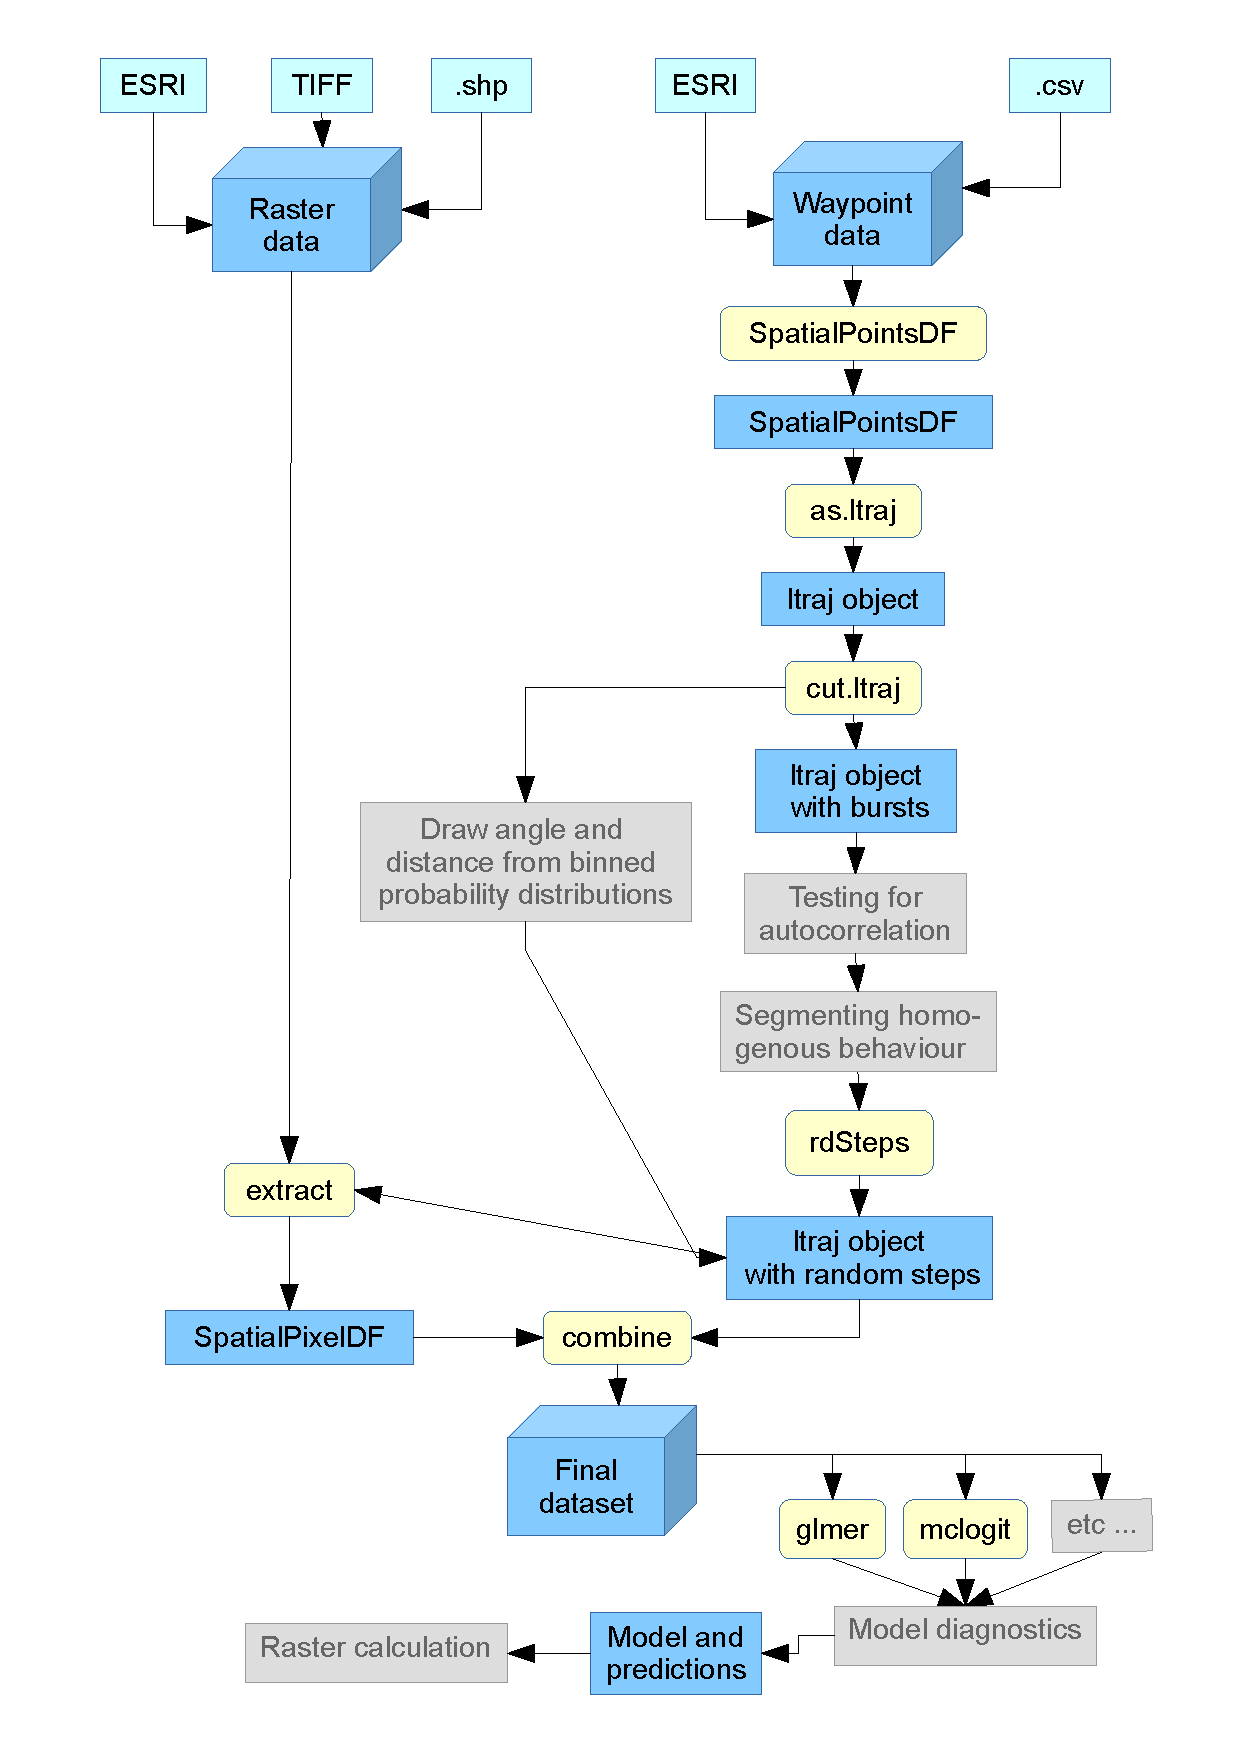
\includegraphics[width=1\textwidth]{Flowchart.pdf} %our perfect workflow!
\caption{Conducting a Step Selection Function using existing R-packages. The yellow boxes show the name of the fucntion applied while the blue boxes provide the type of object or data. Following the arrows a step by step instruction is provided ...}
\label{fig:Flowchart}
\end{figure}




\subsection{Installing and loading Packages}

Before you can actually start using this tutorial for conducting SSF you need to install a bunch of packages in R. Some of them require others so that you have to add all these to your library:

\begin{knitrout}
\definecolor{shadecolor}{rgb}{0.969, 0.969, 0.969}\color{fgcolor}\begin{kframe}
\begin{alltt}
\hlcom{## for implementing SSF}

\hlkwd{install.packages}\hlstd{(}\hlstr{"adehabitatHR"}\hlstd{)}
\hlkwd{install.packages}\hlstd{(}\hlstr{"adehabitatHS"}\hlstd{)}
\hlkwd{install.packages}\hlstd{(}\hlstr{"adehabitatLT"}\hlstd{)}
\hlkwd{install.packages}\hlstd{(}\hlstr{"adehabitatMA"}\hlstd{)}
\hlcom{# Keep fingers off the "adehabitat" package! It is outdated.}

\hlkwd{install.packages}\hlstd{(}\hlstr{"tkrplot"}\hlstd{)}
\hlkwd{install.packages}\hlstd{(}\hlstr{"hab"}\hlstd{,} \hlkwc{repos} \hlstd{=} \hlstr{"http://ase-research.org/R/"}\hlstd{)} \hlcom{# regular}
\hlkwd{install.packages}\hlstd{(}\hlstr{"hab"}\hlstd{,} \hlkwc{repos} \hlstd{=} \hlstr{"http://ase-research.org/R/"}\hlstd{,} \hlkwc{type} \hlstd{=} \hlstr{"source"}\hlstd{)} \hlcom{# for self-compiling}

\hlcom{# for handling raster data}
\hlkwd{install.packages}\hlstd{(}\hlstr{"move"}\hlstd{)}
\hlkwd{install.packages}\hlstd{(}\hlstr{"raster"}\hlstd{)}
\hlkwd{install.packages}\hlstd{(}\hlstr{"rgdal"}\hlstd{)}
\end{alltt}
\end{kframe}
\end{knitrout}

Loading packages:

\begin{knitrout}
\definecolor{shadecolor}{rgb}{0.969, 0.969, 0.969}\color{fgcolor}\begin{kframe}
\begin{alltt}
\hlkwd{require}\hlstd{(hab)}
\hlkwd{require}\hlstd{(adehabitatMA)}
\hlkwd{require}\hlstd{(adehabitatHR)}
\hlkwd{require}\hlstd{(adehabitatHS)}
\hlkwd{require}\hlstd{(adehabitatLT)}

\hlkwd{require}\hlstd{(sp)}
\hlkwd{require}\hlstd{(raster)}
\hlcom{#require(move)}
\hlcom{#require(rgdal)}
\hlcom{#require(tkrplot)}
\end{alltt}
\end{kframe}
\end{knitrout}



\section{Processing the Waypoint Data (or telemetry?)}

\subsection{Loading Waypoint Data (*.csv, ESRI)}%------------------------------------------------------------------------------------------------------

The data for the analysis should be saved in a simple *.csv file format. The table should have column headings in the first line and for each observation include at least the following values: 
\begin{enumerate}
\item{x-coordinate (easting)}
\item{y-coordinate (northing)}
\item{date and/or time}
\item{animal ID}
\end{enumerate}

\noindent Note that the coordinates need to be provided in the same coordinate system and spatial projection as the raster data.

Depending on your analysis you can include further values such as:
\begin{enumerate}
\item{ID for each record}
\item{GPS precision}
\item{other recording parameters such as season}
\item{temperature / elevation at the moment of record}
\item{other values that might be of interest in the further analysis}
\end{enumerate}


\noindent Use the following commands to set your working directory and read the data:
\begin{knitrout}
\definecolor{shadecolor}{rgb}{0.969, 0.969, 0.969}\color{fgcolor}\begin{kframe}
\begin{alltt}
\hlkwd{setwd}\hlstd{(}\hlstr{"/your/working/directory"}\hlstd{)}
\hlstd{xmpl} \hlkwb{=} \hlkwd{read.csv}\hlstd{(}\hlstr{"xmpl.csv"}\hlstd{,} \hlkwc{head}\hlstd{=T)}
\end{alltt}
\end{kframe}
\end{knitrout}

\noindent You can execute \texttt{head(xmpl)} and \texttt{str(xmpl)} to check, whether the data were successfully read.

\subsection{Broken stick model}

\subsection{Creating a Spatial Points Data Frame}%------------------------------------------------------------------------------------------------------
The functions used along the rest of the toolchain can only process data that are stored as objects of class "SpatialPointsDataFrame". This object class stores the coordinates separately and can be created using the according function from package "sp". 

\begin{knitrout}
\definecolor{shadecolor}{rgb}{0.969, 0.969, 0.969}\color{fgcolor}\begin{kframe}
\begin{alltt}
\hlkwd{require}\hlstd{(sp)}

\hlstd{xmpl.spdf} \hlkwb{=} \hlkwd{SpatialPointsDataFrame}\hlstd{(}\hlkwc{coords} \hlstd{= xmpl[,}\hlkwd{c}\hlstd{(}\hlstr{"easting"}\hlstd{,}\hlstr{"northing"}\hlstd{)],} \hlkwc{data} \hlstd{= xmpl)}

\hlkwd{names}\hlstd{(xmpl)}
\end{alltt}
\end{kframe}
\end{knitrout}
In the "coords" argument of the function you should specify the coordinate vectors for your dataset. In our example, we simply assign the two coordinate columns of the example dataset, but you can read the coordinates from a separate file if you want.


\subsection{Creating an ltraj object}%------------------------------------------------------------------------------------------------------
After storing the data in a Spatial Points Data Frame, you now need to connect the single points and turn them into a set of trajectories. This operation is carried out by the function \texttt{as.ltraj} from the "hab" package and produces objects of class "ltraj".
The function \texttt{as.ltraj} requires at least three arguments to work:
\begin{enumerate}
\item{"xy" (x- and y- coordinates for each point)}
\item{"date" (timestamp for each point, given as POSIXct class)}
\item{"id" (the animal id)}
\end{enumerate}

Both coordinates and animal id can easily be adopted from the Spatial Points Data Frame. The timestamp however, is not stored in the required format yet and you therefore need to convert it first:
\begin{knitrout}
\definecolor{shadecolor}{rgb}{0.969, 0.969, 0.969}\color{fgcolor}\begin{kframe}
\begin{alltt}
\hlstd{date} \hlkwb{<-} \hlkwd{as.POSIXct}\hlstd{(}\hlkwd{strptime}\hlstd{(}\hlkwd{paste}\hlstd{(xmpl.spdf}\hlopt{$}\hlstd{LMT_DATE, xmpl.spdf}\hlopt{$}\hlstd{LMT_TIME),} \hlstr{"%d/%m/%Y  %H:%M:%S"}\hlstd{))}
\end{alltt}
\end{kframe}
\end{knitrout}
It is necessary to combine date and time in one POSIXct value. If your dataset already features a POSIXct timestamp, you can skip this step.

Now you can proceed and actually create the ltraj object by executing the following command:
\begin{knitrout}
\definecolor{shadecolor}{rgb}{0.969, 0.969, 0.969}\color{fgcolor}\begin{kframe}
\begin{alltt}
\hlstd{xmpl.ltr} \hlkwb{<-} \hlstd{hab}\hlopt{:::}\hlkwd{as.ltraj}\hlstd{(}\hlkwc{xy} \hlstd{= xmpl.spdf}\hlopt{@}\hlkwc{coords}\hlstd{,} \hlkwc{date} \hlstd{= date,} \hlkwc{id} \hlstd{= xmpl.spdf}\hlopt{$}\hlstd{cat)}
\end{alltt}
\end{kframe}
\end{knitrout}
Two comments to the function as used: By typing \texttt{hab:::as.ltraj} you tell R to use the \texttt{as.ltraj} function from the "hab" package which is speed optimized against its \texttt{adehabitatLT} sibling. Unlike the "xmpl.spdf@coords" promt which works for any SPDF object, the \texttt{xmpl.spdf\$cat} prompt is specific to your dataset. In the example dataset, animal ID's are stored as an integer vector called "cat". If this differs in your dataset and you should change the prompt accordingly.

You now may want to have a closer look at the created ltraj object. Display its structure with by executing \texttt{str(xmpl.ltr)}. 
\begin{knitrout}
\definecolor{shadecolor}{rgb}{0.969, 0.969, 0.969}\color{fgcolor}\begin{kframe}
\begin{alltt}
\hlkwd{str}\hlstd{(xmpl.ltr)}
\end{alltt}
\end{kframe}
\end{knitrout}
When scrolling through the output you will first notice that it consists of 7 elements - the number of individuals in the example dataset. This is because \texttt{as.ltraj()} automatically splits the dataset into subsets one for each individual. We will refine these subsets in the next chapter. Furthermore, the ltraj contains information on the distances and turning angles between consecutive locations.
To get a visual impression of your data you can plot the trajectory for all or for one particular animal:
\begin{knitrout}
\definecolor{shadecolor}{rgb}{0.969, 0.969, 0.969}\color{fgcolor}\begin{kframe}
\begin{alltt}
\hlkwd{plot}\hlstd{(xmpl.ltr)}
\hlkwd{unique}\hlstd{(xmpl.spdf}\hlopt{$}\hlstd{cat)} \hlcom{# prompts a list of all cat ID's. Choose one that you are interested in!}
\hlkwd{plot}\hlstd{(xmpl.ltr,} \hlkwc{id}\hlstd{=}\hlnum{10289}\hlstd{)}
\end{alltt}
\end{kframe}
\end{knitrout}



\subsection{Creating Bursts}%

As described in the previous section, the relocations stored in the ltraj object are already devided into the different individuals. This partition is called a "burst". For analysing the data, there might be the need to create "sub-bursts" for each animal within your trajectory. For example, if the animals were only recorded during the day, the monitoring took place over two consecutive years or the time lag between the relocations differs remarkably, each accumulation of relocations can be defined as a different burst. Looking at those different parts seperately might be necessary for different reasons. The function \texttt{cutltraj} splits the given bursts of your ltraj object into smaller bursts according to a specified criterion. In contrast, the function \texttt{bindltraj} combines the bursts of an object of class "ltraj" with the same attribute "id" to one unique burst. To find out if there are more missing values, you can plot the ltraj object. For that, you need to define the time interval you are looking at. \cite{0.3.162014}


In our example, the locations of the cougars were recorded every 3 hours, starting at 3 AM. The location at midnight is always missing. We now want to split the existing bursts (individuals) into "sub-bursts" where the time lag is smaller than 3 hours. To get an impression about the time lags we plotted the different bursts (individuals). "dt", the time between successive relocations is measured in seconds.

\begin{knitrout}
\definecolor{shadecolor}{rgb}{0.969, 0.969, 0.969}\color{fgcolor}\begin{kframe}
\begin{alltt}
\hlkwd{plotltr}\hlstd{(xmpl.ltr,} \hlstr{"dt/3600/3"}\hlstd{)}
\end{alltt}
\end{kframe}
\end{knitrout}

To cut our data at our desired interval, we need a function which defines "dt". Because we want to keep relocations which are only a few minutes "wrong", we added 10 extra minutes.

\begin{knitrout}
\definecolor{shadecolor}{rgb}{0.969, 0.969, 0.969}\color{fgcolor}\begin{kframe}
\begin{alltt}
\hlstd{foo} \hlkwb{=} \hlkwa{function}\hlstd{(}\hlkwc{dt}\hlstd{) \{}\hlkwd{return}\hlstd{(dt}\hlopt{>} \hlstd{(}\hlnum{3800}\hlopt{*}\hlnum{3}\hlstd{))\}}
\end{alltt}
\end{kframe}
\end{knitrout}

Then we split the object of class ltraj into smaller bursts using \texttt{cutltraj} and the function above. The bursts we had before applying this function still remain.

\begin{knitrout}
\definecolor{shadecolor}{rgb}{0.969, 0.969, 0.969}\color{fgcolor}\begin{kframe}
\begin{alltt}
\hlstd{xmpl.cut} \hlkwb{<-} \hlkwd{cutltraj}\hlstd{(xmpl.ltr,} \hlstr{"foo(dt)"}\hlstd{,} \hlkwc{nextr} \hlstd{=} \hlnum{TRUE}\hlstd{)}
\end{alltt}
\end{kframe}
\end{knitrout}

There are two options of cutting the trajectory depending on nextr. If it is set as FALSE, the burst stops before the first relocation matching the criterion. if it is set as TRUE, it stops after. \cite{0.3.162014}



\subsection{Creating Random Steps}

Given your final bursts we now randomly draw angle and distance from your observed data to get random steps. The angle is taken from the observed position before your starting point of the random step while the distance is taken from the starting point to the next observed position. This means that each burst should at least contain of three observed positions. 
Before applying the function \texttt{rdSteps} you might want to check for correletaion between turning angle and distance. In case your individuals tend to move long distances by turning only in small angles (e.g. a species migrating) but stop for several days for feeding you want to pick the distance and the angle as pairs. If no correlation is found you can pick both variables independently.
To check for this we use the \texttt{plot} function but first have to convert our ltraj object back to a data frame by using \texttt{ld}.
AUTOCORRELATION ???

\begin{knitrout}
\definecolor{shadecolor}{rgb}{0.969, 0.969, 0.969}\color{fgcolor}\begin{kframe}


{\ttfamily\noindent\bfseries\color{errorcolor}{\#\# Error in eval(expr, envir, enclos): could not find function "{}ld"{}}}\end{kframe}
\end{knitrout}

\begin{knitrout}
\definecolor{shadecolor}{rgb}{0.969, 0.969, 0.969}\color{fgcolor}\begin{kframe}
\begin{alltt}
\hlkwd{with}\hlstd{(xmpl.cut.df,} \hlkwd{plot}\hlstd{(dist, rel.angle))}
\end{alltt}


{\ttfamily\noindent\bfseries\color{errorcolor}{\#\# Error in with(xmpl.cut.df, plot(dist, rel.angle)): object 'xmpl.cut.df' not found}}\end{kframe}
\end{knitrout}

\noindent The plot shows a correleation of step length and turning angle and therefore the random steps should be taken as pairs (\texttt{simult = T}). Per default the angle and distance for each random step is drawn from the observed values you provide with \texttt{x}. If your random steps shall be taken from a different dataset you can do so by writting it in \texttt{rand.dist = YourDataSet}. Hereby, you can also specify a distribution for estimating angle and distance. In our case we stick to the same dataset and apply  \texttt{rdSteps}.  

\begin{knitrout}
\definecolor{shadecolor}{rgb}{0.969, 0.969, 0.969}\color{fgcolor}\begin{kframe}
\begin{alltt}
\hlstd{xmpl.steps} \hlkwb{<-} \hlkwd{rdSteps}\hlstd{(}\hlkwc{x} \hlstd{= xmpl.cut,} \hlkwc{nrs} \hlstd{=} \hlnum{10}\hlstd{,} \hlkwc{simult} \hlstd{= T,} \hlkwc{rand.dis} \hlstd{=} \hlkwa{NULL}\hlstd{,}
                      \hlkwc{distMax} \hlstd{=} \hlnum{Inf}\hlstd{,} \hlkwc{reproducible} \hlstd{=} \hlnum{TRUE}\hlstd{,} \hlkwc{only.others} \hlstd{=} \hlnum{FALSE}\hlstd{)}
          \hlcom{# use simult = FALSE if your data is not correlated}
\end{alltt}
\end{kframe}
\end{knitrout}

\noindent The function \texttt{rdSteps} uses some default settings which offer you options to modify your random steps. You can for example, easily change the number of steps taken from the observed data by defining \texttt{nrs} (default is 10) or if you only need steps shorter than a certain value specify \texttt{distMax} to that value (per default all steps are taken). By setting \textt{reproducible = TRUE} a seed is used to get reproducible random steps. If you want to exclude your current individual to draw angle and distance from than set \texttt{only.others = TRUE}.
All in all, \texttt{rdSteps} is very straight forward and computes a lot of useful things for you: 

\begin{knitrout}
\definecolor{shadecolor}{rgb}{0.969, 0.969, 0.969}\color{fgcolor}\begin{kframe}
\begin{alltt}
\hlkwd{head}\hlstd{(xmpl.steps)}
\end{alltt}


{\ttfamily\noindent\bfseries\color{errorcolor}{\#\# Error in head(xmpl.steps): object 'xmpl.steps' not found}}\end{kframe}
\end{knitrout}

\noindent The table still includes your cat id, burst id, the rel.angle and dist of your observed positions. Furthermore, the "case" is provided as categories of 0 and 1 for available and used. The "strata" defines all 10 random steps and the one observed location, so you can later tell your function what to compare.  
Depending on your analysis you might want to compare only your observed positions with the endpoints of your random steps or you want to investigate in the selection of spatial attributes along the path. To do so you find the rel.angle and distance for each random point. Only new coordinates for your random points are missing. Instead two columns provide the differences of your x- and y- coordinates for each random step ("dx" and "dy"). To get new coordinates for your random steps we simply add these differences to your initial coordinates and create two new columns. 

\begin{knitrout}
\definecolor{shadecolor}{rgb}{0.969, 0.969, 0.969}\color{fgcolor}\begin{kframe}
\begin{alltt}
\hlstd{xmpl.steps}\hlopt{$}\hlstd{new_x} \hlkwb{<-} \hlstd{xmpl.steps}\hlopt{$}\hlstd{x} \hlopt{+} \hlstd{xmpl.steps}\hlopt{$}\hlstd{dx}
\hlstd{xmpl.steps}\hlopt{$}\hlstd{new_y} \hlkwb{<-} \hlstd{xmpl.steps}\hlopt{$}\hlstd{y} \hlopt{+} \hlstd{xmpl.steps}\hlopt{$}\hlstd{dy}
\end{alltt}
\end{kframe}
\end{knitrout}

\noindent Thereby, the ???rst observed position will be overwritten as the ???rst random step. That is necessary because there is no random step to compare the ???rst observed position with (angle could not be calculated!). Also the last observed position will be lost for similar reasons (distance could not be calculated!). 
  
\noindent After running this chapter you get your final SpatialPointDataFrame to use with the selection function.
\begin{knitrout}
\definecolor{shadecolor}{rgb}{0.969, 0.969, 0.969}\color{fgcolor}\begin{kframe}
\begin{alltt}
\hlkwd{head}\hlstd{(xmpl.steps)}
\end{alltt}


{\ttfamily\noindent\bfseries\color{errorcolor}{\#\# Error in head(xmpl.steps): object 'xmpl.steps' not found}}\end{kframe}
\end{knitrout}





\section{Processing Spatial Covariates}%----------------------------------------------------------------------------------------------------------------------------
This section explains the handling of spatial parameters that will be tested for selection by the target species. You should store these data in raster files (ESRI *.adf or georeferenced *.tif). These should have the same coordinate system as your telemetry data and should (for time reasons) already be clipped to your study area and. For instructions how to do this in R, please read the GIS instructions from the other group ;)   

\subsection{Load Raster Data (ESRI, *.tif, (*.shp))}%------------------------------------------------------------------------------------------------------

With a simple function stored in the package \textbf{raster} you are able to upload any raster file into R. Examplarily we use raster data on the following parameters for the study area:
\begin{enumerate}
\item{ruggedness of the terrain}
\item{land cover}
\item{canopy cover}
\item{distance to the nearest highway}
\item{distance to the nearest road}
\end{enumerate}

For reading the raster data, three packages are required:
\begin{knitrout}
\definecolor{shadecolor}{rgb}{0.969, 0.969, 0.969}\color{fgcolor}\begin{kframe}
\begin{alltt}
\hlkwd{require}\hlstd{(raster)}
\hlkwd{require}\hlstd{(rgdal)}
\hlkwd{require}\hlstd{(sp)}
\end{alltt}
\end{kframe}
\end{knitrout}

The source files for the raster data can be stored in the working directory or loaded by specifying the exact path. The \texttt{raster()} function is a universal and very powerful tool for loading all kinds of raster data. For reading shapefiles, use the \texttt{readOGR()} function. Below is an example of how to read a set of raster layers.
\begin{knitrout}
\definecolor{shadecolor}{rgb}{0.969, 0.969, 0.969}\color{fgcolor}\begin{kframe}
\begin{alltt}
\hlcom{# First, make sure that your working directory is still the one specified earlier:}
\hlkwd{getwd}\hlstd{()}

\hlcom{# Now read the layers:}
\hlstd{ruggedness} \hlkwb{<-} \hlkwd{raster}\hlstd{(}\hlstr{"ruggedness.adf"}\hlstd{)}
\hlstd{landcover} \hlkwb{<-} \hlkwd{raster}\hlstd{(}\hlstr{"landcover.adf"}\hlstd{)}
\hlstd{canopycover} \hlkwb{<-} \hlkwd{raster}\hlstd{(}\hlstr{"canopycover.adf"}\hlstd{)}
\hlstd{disthighway} \hlkwb{<-} \hlkwd{raster}\hlstd{(}\hlstr{"disthighway.adf"}\hlstd{)}
\hlstd{distroad} \hlkwb{<-} \hlkwd{raster}\hlstd{(}\hlstr{"distroad.adf"}\hlstd{)}
\hlcom{# In the ESRI directory system, raster layers are usually stored in files called "w001001.adf". For demonstration purpose, we copied and renamed them.}
\end{alltt}
\end{kframe}
\end{knitrout}

You can plot the data for a first overview. As this can take a while with large datasets, outcomment the following chunk if you please!
\begin{knitrout}
\definecolor{shadecolor}{rgb}{0.969, 0.969, 0.969}\color{fgcolor}\begin{kframe}
\begin{alltt}
\hlkwd{plot}\hlstd{(ruggedness)}
\hlkwd{plot}\hlstd{(landcover)}
\hlkwd{plot}\hlstd{(canopycover)}
\hlkwd{plot}\hlstd{(disthighway)}
\hlkwd{plot}\hlstd{(distroad)}
\end{alltt}
\end{kframe}
\end{knitrout}

\subsection{Checking for Collinearity}

\subsection{Raster Extraction}
Now that you have generated the random steps and loaded the raster data, you can take the next step and actually connect the trajectories with the spatial covariates. There are different functions that can do this. When choosing one, you need to consider that raster files are large and juggling with them occupies lots of memory and computing power. For this reason we suggest using the \texttt{extract()} function that allows for querying single pixel values without loading the whole source file into working memory. The code for compiling the final dataset involves three steps: Converting the \texttt{xmpl.steps} data frame into a Spatial Points Data frame, extracting the raster values and combining them to the final dataset.
Converting \texttt{xmpl.steps} into a SpatialPointsDataFrame:
\begin{knitrout}
\definecolor{shadecolor}{rgb}{0.969, 0.969, 0.969}\color{fgcolor}\begin{kframe}
\begin{alltt}
\hlstd{xmpl.steps.spdf} \hlkwb{<-} \hlkwd{SpatialPointsDataFrame}\hlstd{(}\hlkwc{coords} \hlstd{= xmpl.steps[,}\hlkwd{c}\hlstd{(}\hlstr{"new_x"}\hlstd{,}\hlstr{"new_y"}\hlstd{)],} \hlkwc{data} \hlstd{= xmpl.steps)}
\end{alltt}
\end{kframe}
\end{knitrout}

Extracting the values from each raster layer:
\begin{knitrout}
\definecolor{shadecolor}{rgb}{0.969, 0.969, 0.969}\color{fgcolor}\begin{kframe}
\begin{alltt}
\hlstd{ruggedness.extr} \hlkwb{<-} \hlkwd{extract}\hlstd{(ruggedness, xmpl.steps.spdf,} \hlkwc{method}\hlstd{=}\hlstr{'simple'}\hlstd{,} \hlkwc{sp}\hlstd{=F,} \hlkwc{df}\hlstd{=T)}
\hlstd{canopycover.extr} \hlkwb{<-} \hlkwd{extract}\hlstd{(canopycover, xmpl.steps.spdf,} \hlkwc{method}\hlstd{=}\hlstr{'simple'}\hlstd{,} \hlkwc{sp}\hlstd{=F,} \hlkwc{df}\hlstd{=T)}
\hlstd{disthighway.extr} \hlkwb{<-} \hlkwd{extract}\hlstd{(disthighway, xmpl.steps.spdf,} \hlkwc{method}\hlstd{=}\hlstr{'simple'}\hlstd{,} \hlkwc{sp}\hlstd{=F,} \hlkwc{df}\hlstd{=T)}
\hlstd{distroad.extr} \hlkwb{<-} \hlkwd{extract}\hlstd{(distroad, xmpl.steps.spdf,} \hlkwc{method}\hlstd{=}\hlstr{'simple'}\hlstd{,} \hlkwc{sp}\hlstd{=F,} \hlkwc{df}\hlstd{=T)}
\hlstd{landcover.extr} \hlkwb{<-} \hlkwd{extract}\hlstd{(landcover, xmpl.steps.spdf,} \hlkwc{method}\hlstd{=}\hlstr{'simple'}\hlstd{,} \hlkwc{sp}\hlstd{=F,} \hlkwc{df}\hlstd{=T)}
\end{alltt}
\end{kframe}
\end{knitrout}
The extraction is done separately for each layer. The option \texttt{method = 'simple'} extracts value from nearest cell whereas \texttt{method = 'bilinear'} interpolates from the four nearest cells. You can adjust this option according to the resolution of your dataset and ecological considerations. \texttt{df=T} returns the result as a data frame and \texttt{sp=F} ensures that the output is not added to the original dataset right away. 

Automatically adding the extracted values to the original dataset sounds like a handy option. For two reasons we do not use it here: Firstly, we want to set the column names manually for not ending up with several columns called "w001001". Secondly, our data include a categorial covariate (landcover) that we want to reclassify and flag as a factor.

This is the code for compiling the final dataset:
\begin{knitrout}
\definecolor{shadecolor}{rgb}{0.969, 0.969, 0.969}\color{fgcolor}\begin{kframe}
\begin{alltt}
\hlstd{xmpl.steps.spdf}\hlopt{$}\hlstd{ruggedness} \hlkwb{<-} \hlstd{ruggedness.extr[,}\hlnum{2}\hlstd{]}
\hlstd{xmpl.steps.spdf}\hlopt{$}\hlstd{canopycover} \hlkwb{<-} \hlstd{canopycover.extr[,}\hlnum{2}\hlstd{]}
\hlstd{xmpl.steps.spdf}\hlopt{$}\hlstd{disthighway} \hlkwb{<-} \hlstd{disthighway.extr[,}\hlnum{2}\hlstd{]}
\hlstd{xmpl.steps.spdf}\hlopt{$}\hlstd{distroad} \hlkwb{<-} \hlstd{distroad.extr[,}\hlnum{2}\hlstd{]}

\hlcom{# The landcover covariate comes coded in integers between 0 an 10 and is by default (mis)interpreted as an integer string. }
\hlkwd{unique}\hlstd{(landcover.extr[,}\hlnum{2}\hlstd{])}
\hlcom{# Re-classifying landcover:}
\hlstd{xmpl.steps.spdf}\hlopt{$}\hlstd{landcover} \hlkwb{<-} \hlkwd{as.factor}\hlstd{(}
    \hlkwd{ifelse}\hlstd{(landcover.extr[,}\hlnum{2}\hlstd{]} \hlopt{==} \hlnum{0}\hlstd{,}\hlstr{"NA"}\hlstd{,}
    \hlkwd{ifelse}\hlstd{(landcover.extr[,}\hlnum{2}\hlstd{]} \hlopt{<} \hlnum{5}\hlstd{,} \hlstr{"forest"}\hlstd{,}
    \hlkwd{ifelse}\hlstd{(landcover.extr[,}\hlnum{2}\hlstd{]} \hlopt{<} \hlnum{8}\hlstd{,} \hlstr{"open"}\hlstd{,}\hlstr{"NA"}\hlstd{))))}
\end{alltt}
\end{kframe}
\end{knitrout}
Now your final dataset should be ready for analysis. Examine it:  
\begin{knitrout}
\definecolor{shadecolor}{rgb}{0.969, 0.969, 0.969}\color{fgcolor}\begin{kframe}
\begin{alltt}
\hlkwd{head}\hlstd{(xmpl.steps.spdf)}
\end{alltt}
\end{kframe}
\end{knitrout}




\section{Final SSF Model}

Using the function \texttt{cs.} we get comparable values for each predictor. The according equation is: 
\[
\displaystyle f(x) = (x - mean)/sd(x)
\]

\section{Acknowledgements}
Don't forget to thank TeX and R and other opensource communities if you use their products! The correct way to cite R is shown when typing ``\texttt{citation()}'', and ``\texttt{citation("mgcv")}'' for packages.

Special thanks to \ding{164} \ding{170} Simone \ding{170}\ding{170}\ding{170} \ding{164}\ding{165}\ding{95}! You were our best team member! \ding{96}

Save Models!

\section{Appendix}

Session Info:
\begin{knitrout}
\definecolor{shadecolor}{rgb}{0.969, 0.969, 0.969}\color{fgcolor}\begin{kframe}
\begin{verbatim}
## R version 3.1.1 (2014-07-10)
## Platform: i386-w64-mingw32/i386 (32-bit)
## 
## locale:
## [1] LC_COLLATE=English_United Kingdom.1252 
## [2] LC_CTYPE=English_United Kingdom.1252   
## [3] LC_MONETARY=English_United Kingdom.1252
## [4] LC_NUMERIC=C                           
## [5] LC_TIME=English_United Kingdom.1252    
## 
## attached base packages:
## [1] stats     graphics  grDevices utils     datasets  methods   base     
## 
## other attached packages:
## [1] knitr_1.7
## 
## loaded via a namespace (and not attached):
## [1] evaluate_0.5.5 formatR_1.0    highr_0.4      stringr_0.6.2  tools_3.1.1
\end{verbatim}
\end{kframe}
\end{knitrout}

\bibliography{References}{}
\bibliographystyle{plain}


\end{document}
